\documentclass[12pt,letter]{aastex}
\usepackage[hyphens]{url}
%\usepackage[breaklinks]{hyperref}   %This is the key package which allows url wrapping.
%\usepackage[draft]{hyperref}
%\usepackage[hyphenbreaks]{breakurl}
\usepackage{longtable}
\usepackage{amsmath,amssymb,multirow,dcolumn,fancyhdr,charter,graphicx}
\usepackage{graphics}
\usepackage{xspace}
\usepackage{color,ulem,epstopdf}
\newcommand{\x}{\sout}
\newcommand{\w}{\color{red}}
\newcommand{\vdag}{(v)^\dagger}
\def\memohr#1{\color{blue}$HR[${\bf #1}$]$ \color{black}}
\def\memoas#1{\color{red}$AS[${\bf #1}$]$ \color{black}}
\def\commentas#1{\color{purple}$AS[${\bf #1}$]$ \color{black}}
\def\refr#1{{\bf #1}}
\usepackage{tikz}
\def\checkmark{\tikz\fill[scale=0.4](0,.35) -- (.25,0) -- (1,.7) -- (.25,.15) -- cycle;} 

%commands
\newcommand{\reb}{{\sc \tt REBOUND}\xspace}
\newcommand{\whfast}{{\sc \tt WHFAST}\xspace}
\newcommand{\ias}{{\sc \tt IAS15}\xspace}
\newcommand{\emcee}{{\sc \tt EMCEE}\xspace}
\newcommand{\Lagr}{\mathcal{L}}
\newcommand{\kep}{{\it Kepler}\xspace}

%journal abbreviations
      
\date{Draft version: \today}

\begin{document}
\section{Introduction}

Proposed sections in the introduction:
\begin{enumerate}
\item Exoplanet detection -- Dominant detection methods = Transit, RV. Basic statistics of exoplanets discovered by Kepler Space Telescope. 
\item Planet Formation -- MMSN, Core accretion/GI models, Planetesimal Formation, Nice Model. 
\item Planet Dynamics -- Migration, Mean Motion Resonance, Stability.
\item Numerical Integration -- Hamiltonian Dynamics, Close Encounters, etc. 
\end{enumerate}

Below I am going to elaborate on planet dynamics. 

\section{Planet Dynamics}
\subsection{Migration}
It is well known that planetary systems form from a collection gas and dust known as a protoplanetary disk. 


\subsection{Mean Motion Resonance (MMR)}
Planets can be in MMR when the orbital period of one planet is an integer ratio of another. 
Like other types of resonance that occur in nature, MMR results in the amplitude growth of various quantities characterizing the system, like eccentricity, semi-major axis and the longitude of pericentre \citep{SSD1999}. 
As a result, the presence of MMR can strongly affect the formation, evolution and longterm stability of planetary systems in a diversity of ways.
For example, Kirkwood gaps are unstable regions in the asteroid belt carved by MMR with Jupiter, while Pluto and Neptune are protected from colliding due to MMR, even though their orbits overlap. 

There are two resonant angles related to every $p:q$ MMR (where $p$ and $q$ are integers):
\begin{align*}
\begin{split}
\phi_1 &= p\lambda_1 - q\lambda_2 + \omega_1 \\
\phi_2 &= p\lambda_1 - q\lambda_2 + \omega_2 
\end{split}
\end{align*}
where $\lambda$ is the mean longitude and $\omega$ is the longitude of periapse. 
For planets to be in MMR at least one resonant angle is librating.
%, however there are exceptions to this rule.
%For example, planets with commensurate period ratios are not required to be in MMR, and planets a few percent away from period commensurability can be found to be in MMR \citep[e.g.][]{Lee2002}. 
%In addition, circulating resonant angles can be associated with planets in MMR while librating resonant angles can be associated with planets not in MMR \citep{Delisle2012}.
%As a result, it can be difficult to constrain the formation histories of discovered planetary systems. 



\begin{figure}
\centering
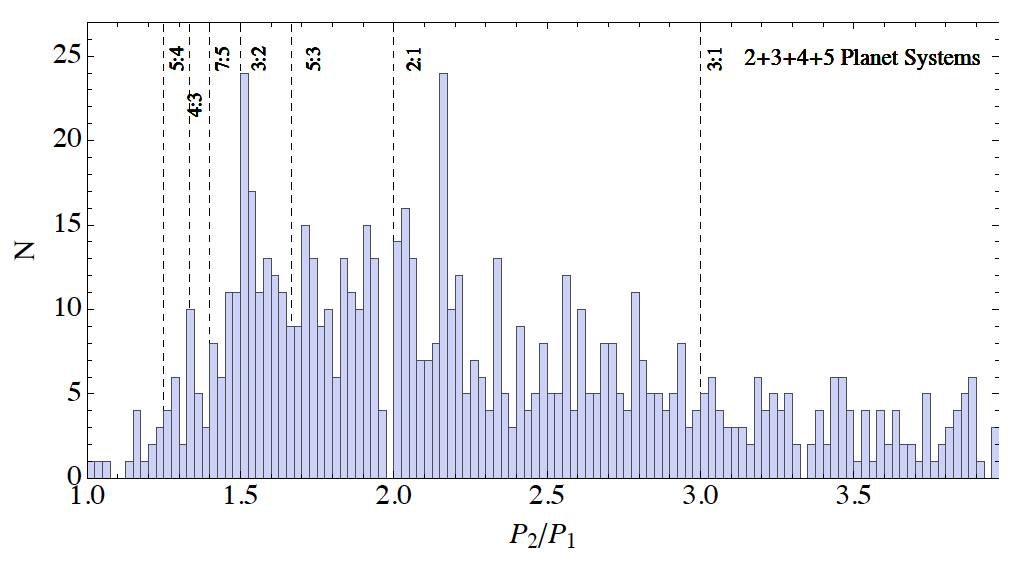
\includegraphics[width=1.00\textwidth]{Figures/KeplerPeriods.png}
\caption{
\footnotesize Period ratios of Kepler planets, image from \citet{Goldreich2014}.}
\label{fig:KepMMR}
\end{figure}

Of particular interest are the planetary systems discovered by \kep.
Figure~\ref{fig:KepMMR} shows the distribution of \kep period ratios, along with the locations of first and second order MMR. 
As can be seen, statistical excesses of planets exist just wide of the 2:1 and 3:2 MMR \citep{Lissauer2011,Fabrycky2014,Steffen2015}.
If planets are to get captured in MMR it is expected that they would be captured in these since MMR strength is proportional to $e^{p-q}$ \memoas{need citation}.
The most popular dissipative mechanisms to explain these observed near-resonant systems are tidal \citep{LithwickWu2012, Batygin2013, Delisle2014},  protoplanetary \citep{Rein2012b, Baruteau2013, Goldreich2014}, and planetesimal \citep{Moore2013, Chatterjee2015}. 
The formation implications for each mechanism are different, and no clear consensus has yet emerged.

%Structure of MMR -- pendulum model, Separatrix, libration of resonant angles. 
%With the exception of a these statistically significant excesses at first order resonances, the period distribution of planets is to first order uniform.

\begin{enumerate}
\item Excess of Kepler planets near MMR (plot), but most planets are far from MMR. 
\item Theory dictates that a) planets embedded in a protoplanetary disk tend to migrate and b) migrating planets should be captured in MMR. First order resonances are dominant modes of capture, as the strength of the resonance goes as $e^{p-q}$. Evidence is mounting that this picture is far more complicated than originally believed (e.g. Jeff's paper says planets don't migrate). 
\item If planets are trapped in MMR after the dispersal of the protoplanetary disk, there are only a few mechanisms able to transport planets from MMR -- tides, planet-planet scattering, and planetesimals. 
\end{enumerate}

\subsection{Stability}

\bibliographystyle{apj}
\bibliography{intro_ver1.bib}

\end{document}

